\documentclass[a4paper, 10pt]{article} % For LaTeX2e
\usepackage{amsmath}
\usepackage{amssymb}
\usepackage[colorlinks=true,
            linkcolor=red,
            urlcolor=blue,
            citecolor=gray]{hyperref}
\usepackage[utf8]{inputenc}
\usepackage[T1]{fontenc}
\usepackage{lmodern}
\usepackage[frenchb]{babel}
%\usepackage{times}
\usepackage{graphicx}
\usepackage{color}
\usepackage[usenames,dvipsnames,svgnames,table]{xcolor}
\usepackage{multirow}
\usepackage[authoryear,round]{natbib}
\usepackage{bbm}
\usepackage{latexsym}
\usepackage{epsfig}
\usepackage{subfigure}
\usepackage{placeins}
\usepackage{algorithmic}
\usepackage{algorithm}
\usepackage{rotating}
\usepackage{hyperref}
\usepackage{fancyhdr}
\usepackage{alltt}
\usepackage[left=2cm,right=2cm,top=3cm,bottom=2cm]{geometry}

% TikZ
\usepackage{pgf}
\usepackage{tikz}
\usetikzlibrary{arrows}

% Where can LaTeX find figures ?
\graphicspath{{images/}}

% PDF informations
%-----------------------------------------------------------------
\hypersetup{%
  pdfstartview=FitH,
  colorlinks=true,
  pdfborder=0 0 0,
  pdftitle    = {INC Spring2014 : Spécification du protocole de communication avec le périphérique},
  pdfsubject  = {INC, ECP, LISA},
  pdfauthor   = {Xavier Lagorce,Laurent Cabaret},
  pdfkeywords = {INC, Spring2014, protocole, communication, enocean}}

%\usepackage{vmargin}            % red?finir les marges
%\setmarginsrb{3cm}{3cm}{3cm}{3cm}{1cm}{2cm}{1cm}{2cm}

% Configuration des headers
\pagestyle{fancy}
%\fancyhead{} %Effacer les headers
\lhead{Projet Enhanced Light Bike}
\rhead{Communication avec la centrale du vélo}

\newcommand{\saut}{\vspace{0.5cm}}
\newcommand{\rien}{-}
\newcommand{\numero}{n\textsuperscript{o}}

\title{{\huge Enhanced Light Bike}\vspace{0.5cm}\\Spécifications du protocole de communication avec la centrale du vélo}
\author{\href{mailto:Xavier.Lagorce@crans.org}{Xavier Lagorce}\\\href{mailto:laurent.cabaret@ecp.fr}{Laurent Cabaret}}
\date{3 Mars 2014 - v1.00\\Ce document est sujet à modifications}

\begin{document}

\maketitle

\vspace{1cm}

\tableofcontents
\newpage

\section{Introduction}

Le présent document spécifie le protocole de communication utilisé entre l'hôte (la centrale)
et le périphérique (Système d'éclairage).

\section{Médium}

La communication entre l'hôte et le périphérique se fera à travers une liaison propriétaire fournissant un port série (Tx et Rx) \footnote{Cela correspond au type de liaison série utilisée lors de la formation Arduino.} ainsi que 2 alimentations 5V et 12V (variable selon votre application - prévenez l'équipe enseignante de vos besoins le plus tôt possible) et une masse.

\saut

\subsection{Liaison série}
La liaison série aura les paramètres suivants\footnote{Ces paramètres sont le plus souvent regroupés
sous l'appellation 9600/8N1} :
\begin{itemize}
  \item vitesse de communication : 9600 bps
  \item 8 bits de données
  \item pas de bit de parité
  \item 1 bit de stop
\end{itemize}

\subsection{Connecteur}

Nous allons utiliser un connecteur à dix contacts 5x2 

\begin{center}
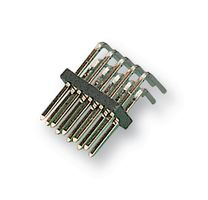
\includegraphics[scale=0.5]{HE10.jpg}
\end{center}

dont le brochage devra obligatoirement être le suivant :

\begin{center}
\begin{tabular}{r|c||c|l}
GND&1&10&Nc\\
5V&2&9&Nc\\
12V&3&8&Nc\\
TxO&4&7&Nc\\
RxI&5&6&Nc\\
\end{tabular}
\end{center}


\begin{itemize}
\item TxO sera connecté au Tx de l'arduino
\item RxI sera connecté au Rx de l'arduino
\end{itemize}


Ce point étant critique, il est obligatoire de contacter le responsable du design de la communication de la centrale\footnote{laurent.cabaret@ecp.fr} avant l'impression  de votre carte prototype.
En effet le sens du connecteur (Top/Bottom/...) du coté centrale n'est pas modifiable.

Nous rappelons que lors de la soutenance il faudra très rapidement pouvoir connecter la centrale a votre système sans démontage de plus de 5s. Tout problème dans cette communication sera considéré comme une erreur de conception.

%Références Farnell : 2293829 ou 2009455
Références Radiospares : à définir.

Pour simplifier votre travail une bibliothèque de composant est mise a votre disposition sur ged dans composants fournis sous le nom de \emph{LibConnecteur}

\section{Protocole}

\subsection{Format des commandes}

Une commande envoyée par l'hôte sera une chaîne de caractères ASCII lisibles par un humain. elle aura la
forme suivante :
\begin{center}
  \verb|SSDV<cr>|
\end{center}

où :
\begin{itemize}
  \item \verb|SS| est à remplacer par les lettres codant un type de capteur particulier.
  \item \verb|D| est à remplacer par le numéro du capteur ou de l'actionneur.
  \item \verb|V| code la valeur de l'information 
  \begin{itemize}
	\item  U pour front montant (bouton appuyé),
	\item  D pour front descendant(bouton relaché), 
	\item  H pour position haute (lampe), 
	\item  L pour position basse (lampe).  
  \end{itemize}
  \item \verb|<cr>|\footnote{<cr> est un caractère spécial : carriage return ou retour chariot \href{http://fr.wikipedia.org/wiki/American_Standard_Code_for_Information_Interchange}{Code Acsii}}
\end{itemize}

\subsection{Liste des commandes}
Le bouton "enocean" sera le premier capteur sur le vélo il reçoit donc le nom BT1
La lampe est le premier actionneur sur le vélo il reçoit donc le nom LI1.

Liste des commandes possibles est en provenance de la centrale est :
\begin{itemize}
	
\item 	\verb|BTxU| : Le bouton \numero x a été appuyé.
	
\item 	\verb|BTxD| : Le bouton \numero x a été relaché.

\item 	\verb|LIx?| : Demande d'état de la lampe \numero.
\end{itemize}

Liste des réponses en provenance de la lampe :
\begin{itemize}
\item 	\verb|LIxK| : La lampe \numero x confirme qu'elle a bien reçu le message.

\item 	\verb|LIxH| : La lampe \numero x est en position haute.

\item 	\verb|LIxL| : La lampe \numero x est en position basse.
\end{itemize}


\section{Exemple type d'une conversation}
\begin{center}
\begin{tabular}{|c|c|p{6cm}|}
\hline
Centrale&ELBike&\\
\hline
\hline
\verb|LI1?<cr>|&\rien& La centrale demande : Position de la lampe ?\\
\rien&\verb|LI1H<cr>|& La lampe répond : Haut\\
\hline
\vdots&\vdots& 	\\
\hline
\verb|LI1?<cr>|&\rien& La centrale demande : Position de la lampe ?\\
\rien&\verb|LI1H<cr>|& La lampe répond : Haut\\
\hline
\verb|BTxU<cr>|&\rien& La centrale indique que le bouton a été enfoncé\\
\rien&\verb|LI1K<cr>|& La lampe répond : Bien reçu\\
\hline
\verb|BTxD<cr>|&\rien& La centrale indique que le bouton a été relaché\\
\rien&\verb|LI1K<cr>|& La lampe répond : Bien reçu\\
\hline
\verb|LI1?<cr>|&\rien& La centrale demande : Position de la lampe ?\\
\rien&\verb|LI1L<cr>|& La lampe répond : Basse\\
\hline
\vdots&\vdots& 	\\
\hline
\verb|LI1?<cr>|&\rien& La centrale demande : Position de la lampe ?\\
\rien&\verb|LI1H<cr>|& La lampe répond : Haut\\
\hline
\end{tabular}
\end{center}


\end{document}

